\documentclass[11pt,a4paper]{article}

% ── encoding & language ──────────────────────────────────────────────────────
\usepackage[utf8]{inputenc}
\usepackage[T1]{fontenc}
\usepackage[spanish]{babel}

% ── typography ───────────────────────────────────────────────────────────────
\usepackage{lmodern}
\usepackage{helvet}
\renewcommand{\familydefault}{\sfdefault}
\usepackage{microtype}
\usepackage{setspace}
\onehalfspacing

% ── page layout ──────────────────────────────────────────────────────────────
\usepackage[top=2.5cm,bottom=2.5cm,left=2.5cm,right=2.5cm]{geometry}

\usepackage{amsmath,amssymb}
\usepackage{booktabs}
\usepackage{array}
\usepackage{makecell}
\usepackage{caption}
\usepackage{graphicx}
\graphicspath{{output/figures/}}
\usepackage[colorlinks=true, linkcolor=blue, urlcolor=blue]{hyperref}
\usepackage{float}
\usepackage{xcolor}
\usepackage{tcolorbox}
\usepackage{enumitem}

\addto\captionsspanish{%
  \renewcommand{\contentsname}{Índice}%
}

% Caja explicativa reusable
\newtcolorbox{ideabox}[1]{
  colback=blue!5!white,
  colframe=blue!50!black,
  title=#1,
  fonttitle=\bfseries,
  boxrule=0.8pt,
  arc=2pt,
  left=8pt,right=8pt,
  before skip=10pt,after skip=10pt
}

\newtcolorbox{lectura}[1]{
  colback=green!4!white,
  colframe=green!40!black,
  title=#1,
  fonttitle=\bfseries,
  boxrule=0.8pt,
  arc=2pt,
  left=8pt,right=8pt,
  before skip=10pt,after skip=10pt
}

\newtcolorbox{warning}[1]{
  colback=orange!8!white,
  colframe=orange!70!black,
  title=#1,
  fonttitle=\bfseries,
  boxrule=0.8pt,
  arc=2pt,
  left=8pt,right=8pt,
  before skip=10pt,after skip=10pt
}

\setlength{\parindent}{0pt}
\setlength{\parskip}{8pt}

\begin{document}

% ── Portada ─────────────────────────────────────────────────────────────────
\begin{titlepage}
\centering
\vspace*{3\baselineskip}
{\Huge\bfseries Guía de lectura de la tesis}\par
\vspace{0.5\baselineskip}
{\Large \textit{Cómo interpretar cada tabla y figura}}\par
\vspace{2\baselineskip}
{\large Impacto de la disponibilidad de ChatGPT en el desarrollo \\
de software orientado a Ciencia de Datos (2020--2023)}\par
\vspace{3\baselineskip}
\rule{0.6\textwidth}{0.5pt}\par
\vspace{2\baselineskip}
{\normalsize Documento complementario a la tesis principal}\par
\vspace{0.5\baselineskip}
{\normalsize Nicho Rosado, Jesus Alberto \quad \textbar \quad Janampa Aparicio, Karl Willem}\par
\vspace{0.5\baselineskip}
{\normalsize Asesor: Quispe Rojas, Alexander Wilder}\par
\vspace{4\baselineskip}
{\small Lima, 2026}\par
\vfill
\end{titlepage}

\tableofcontents
\clearpage

% ════════════════════════════════════════════════════════════════════════════
\section{Para qué sirve este documento}

Esta guía explica, paso a paso, qué muestra cada cuadro y cada figura de la tesis y cómo interpretarlos. Está pensada para que cualquier lector —aunque no tenga formación en econometría avanzada— pueda entender qué dice tu trabajo y por qué lo que encontraste tiene valor.

\begin{ideabox}{Cómo está organizado}
\begin{itemize}[leftmargin=*]
  \item \textbf{Parte I (Secciones 2--3):} la pregunta de investigación y los datos.
  \item \textbf{Parte II (Sección 4):} conceptos clave de econometría que aparecen en toda la tesis.
  \item \textbf{Parte III (Sección 5):} los tres métodos econométricos en lenguaje simple.
  \item \textbf{Parte IV (Secciones 6--15):} cómo leer cada cuadro y figura, una por una.
  \item \textbf{Parte V (Sección 16):} resumen ejecutivo de los hallazgos.
\end{itemize}
\end{ideabox}

% ════════════════════════════════════════════════════════════════════════════
\section{La pregunta de investigación}

\textbf{Pregunta central:} ¿La disponibilidad pública de ChatGPT (lanzado el 30 de noviembre de 2022) aumentó la cantidad de desarrolladores activos en GitHub en los países donde el servicio fue accesible, comparado con los países donde no estuvo disponible?

\textbf{¿Por qué importa?} Si la respuesta es sí, significa que esta nueva tecnología de IA generativa no solo es popular —también está cambiando objetivamente la dinámica de la industria del software. Esto tiene implicaciones para empresas, gobiernos y la educación tecnológica.

\textbf{La hipótesis:} El efecto debería ser positivo y más fuerte en lenguajes con vasta documentación técnica (como Python y JavaScript), porque ChatGPT fue entrenado con más texto en esos lenguajes y por tanto los maneja mejor.

% ════════════════════════════════════════════════════════════════════════════
\section{Los datos en una página}

\textbf{Fuente:} GitHub Innovation Graph, una base pública que GitHub mantiene con métricas agregadas de actividad de desarrollo por país, lenguaje y trimestre.

\textbf{Variable de interés:} \textit{unique pushers} por cada 100\,000 habitantes — el número de programadores únicos que al menos subieron código a GitHub en un trimestre dado, normalizado por población. Esto es una medida \textit{per cápita} de actividad de desarrollo.

\textbf{Ventana de análisis:} 16 trimestres, desde Q1-2020 hasta Q4-2023.

\textbf{Lenguajes analizados:} los 10 más populares en ciencia de datos según rankings consultados: \textit{C, C\#, C++, Go, Java, JavaScript, PHP, Python, Ruby, TypeScript}.

\textbf{Países:} 159 países en total ---- 130 con acceso a ChatGPT (\textbf{grupo tratado}) y 29 sin acceso al momento del lanzamiento (\textbf{grupo de control}). Los países sin acceso son aquellos donde ChatGPT estuvo restringido (China, Rusia, Irán, Corea del Norte, etc.).

\textbf{Tamaño total:} 25\,440 observaciones trimestrales (159 países $\times$ 10 lenguajes $\times$ 16 trimestres).

\begin{warning}{Por qué Hong Kong{,} EU y Kosovo se excluyen}
La Unión Europea (EU) aparece como agregado, lo que duplicaría las observaciones de los países miembros. Kosovo (XK) no tiene código procesable por las librerías de geolocalización. Hong Kong (HK) mostraba un nivel atípicamente alto de \textit{unique pushers} que distorsionaría las estimaciones. Su exclusión es metodológica, no política.
\end{warning}

% ════════════════════════════════════════════════════════════════════════════
\section{Conceptos clave en una página}

Antes de entrar en los métodos, conviene fijar siete conceptos que vas a ver mencionados muchas veces en la tesis. Si los entiendes acá, no tendrás que buscarlos en internet cada vez que aparezcan.

\subsection*{1. ATT (Average Treatment Effect on the Treated)}

\textbf{Definición.} El ATT es el efecto causal promedio que el tratamiento tuvo sobre las unidades que efectivamente lo recibieron. Es la diferencia esperada entre lo que pasó con los 130 países tratados y lo que les habría pasado si ChatGPT nunca hubiera estado disponible.

\textbf{Ejemplo en esta tesis.} Cuando el Cuadro 3 reporta ``JavaScript: SDID = $8{,}303$'', significa que la disponibilidad de ChatGPT causó un aumento promedio de 8{,}303 \textit{unique pushers} por cada 100\,000 habitantes en los 130 países con acceso al servicio.

\textbf{Para qué se usa.} Es la magnitud central que esta tesis estima. Cada celda numérica de los Cuadros 3, 4, 5 y 6 es un ATT (o un ATT placebo en el caso del Cuadro 6).

\subsection*{2. Contrafactual}

\textbf{Definición.} El contrafactual es lo que habría pasado en un mundo paralelo donde el tratamiento no ocurrió. Como nunca se puede observar directamente, los métodos econométricos lo aproximan a partir del grupo de control.

\textbf{Ejemplo en esta tesis.} En las Figuras 5--14, paneles (a), (c) y (e), la línea roja es el contrafactual: el grupo tratado ``sintético'' construido a partir de los países sin acceso a ChatGPT. La diferencia entre la línea azul (lo observado) y la línea roja (lo que habría sucedido sin tratamiento) es el efecto causal.

\textbf{Para qué se usa.} La calidad con la que el método reconstruye el contrafactual determina la credibilidad del efecto. Por eso se comparan tres métodos: DiD, CS y SDiD construyen contrafactuales distintos.

\subsection*{3. Tendencias paralelas}

\textbf{Definición.} Es el supuesto crítico del DiD: en ausencia del tratamiento, los grupos tratado y de control habrían evolucionado de forma paralela en el tiempo. Si esto no se cumple ---por ejemplo, si los países tratados ya venían creciendo más rápido antes del lanzamiento---, el DiD confunde el efecto del tratamiento con una tendencia preexistente.

\textbf{Ejemplo en esta tesis.} En el panel (a) Tendencias DiD de cualquier Figura 5--14, si las líneas azul y roja no son paralelas \textbf{antes} de Q4-2022, el supuesto se viola. Por eso el SDiD asigna pesos a los donantes: construye un control sintético cuyas tendencias pre-tratamiento coinciden con las del tratado.

\textbf{Para qué se usa.} Es lo que separa un buen contrafactual de uno sesgado. Los métodos sintéticos (CS, SDiD) son preferibles al DiD cuando el supuesto de tendencias paralelas falla.

\subsection*{4. Error estándar e intervalo de confianza}

\textbf{Definición.} El error estándar (SE) mide la incertidumbre del estimador: cuánto variaría el ATT si pudiéramos repetir el estudio con otra muestra de países. El intervalo de confianza al 95\,\% se construye aproximadamente como $\text{ATT} \pm 2 \times \text{SE}$ y representa el rango plausible del efecto verdadero.

\textbf{Ejemplo en esta tesis.} En el Cuadro 3, Python SDID muestra ATT $= 4{,}525$ con SE $= 1{,}321$ (entre paréntesis). El intervalo de confianza al 95\,\% es aproximadamente $[4{,}525 - 2{,}642;\ 4{,}525 + 2{,}642] = [1{,}88;\ 7{,}17]$. Como no incluye cero, el efecto es estadísticamente distinto de cero.

\textbf{Para qué se usa.} Mide cuán preciso es el ATT estimado. Un SE chico significa más confianza; uno grande, mayor incertidumbre. Es lo que aparece entre paréntesis en \textbf{todos} los cuadros de resultados.

\subsection*{5. P-valor y significancia estadística}

\textbf{Definición.} El p-valor es la probabilidad de observar un efecto al menos tan grande como el estimado, suponiendo que el efecto verdadero fuera cero. Un p-valor pequeño indica que el resultado es poco probable por azar, lo que se llama ``significancia estadística''.

\textbf{Ejemplo en esta tesis.} Las estrellas en el Cuadro 3 traducen p-valores: $*$ p$<$0{,}10; $**$ p$<$0{,}05; $***$ p$<$0{,}01. JavaScript SDID con $***$ significa que la probabilidad de observar un ATT de 8{,}303 o más por puro azar es menor a 1\,\%.

\textbf{Para qué se usa.} Permite decidir si un efecto es ``detectable'' o no. \textit{Cuidado}: significancia estadística no es lo mismo que importancia económica o práctica ---un efecto puede ser muy significativo pero pequeño en magnitud, y viceversa.

\subsection*{6. Bootstrap}

\textbf{Definición.} El bootstrap es una técnica para estimar la incertidumbre de un estimador sin asumir una distribución teórica. Funciona remuestreando los datos con reemplazo muchas veces, recalculando el estimador en cada muestra, y midiendo cuánto varía.

\textbf{Ejemplo en esta tesis.} En la sección de Inferencia, se hacen 100 replicaciones bootstrap para DiD y SDiD, y 2\,000 para CS. En cada replicación se vuelven a sortear los países con reemplazo y se recalcula el ATT; el SE final es la desviación estándar de esas estimaciones.

\textbf{Para qué se usa.} Es la forma de calcular los SE cuando la fórmula teórica es complicada o cuando los supuestos clásicos (normalidad, homoscedasticidad) no aplican. Los números entre paréntesis de los Cuadros 3, 4 y 5 vienen de bootstrap.

\subsection*{7. Identificación causal versus correlación}

\textbf{Definición.} Correlación significa que dos variables se mueven juntas. Identificación causal significa probar que una variable es la \textbf{causa} del cambio en la otra, descartando otras explicaciones. Para identificar causalidad se necesita un diseño de investigación que aísle el efecto del tratamiento del resto.

\textbf{Ejemplo en esta tesis.} Que la actividad de GitHub haya aumentado después de noviembre de 2022 NO prueba que ChatGPT la causó: pudo ser una tendencia post-pandemia, o crecimiento del internet global. La estrategia DiD/SC/SDiD usa el grupo de control (países sin acceso) para identificar: lo que distingue al efecto causal es que aparece solo en los países con acceso, no en los demás durante el mismo período.

\textbf{Para qué se usa.} Es lo que diferencia esta tesis de un simple análisis descriptivo. Sin identificación causal, las recomendaciones de política no tendrían base empírica.

\begin{ideabox}{Cómo usar esta sección}
Si en algún momento del documento aparece un término que no entiendes (ATT, contrafactual, p-valor, etc.), regresa acá. Esta sección es la ``hoja de referencia'' para que ninguna celda numérica te quede en el aire.
\end{ideabox}

% ════════════════════════════════════════════════════════════════════════════
\section{Los tres métodos en lenguaje simple}

La tesis usa tres métodos econométricos para estimar el efecto causal del lanzamiento de ChatGPT. La idea común es la misma: \textbf{comparar lo que pasó en los países con ChatGPT contra lo que habría pasado si no hubieran tenido acceso}. Como no podemos observar este escenario contrafactual directamente, lo aproximamos con los países sin acceso.

\subsection{Método 1: Diferencias en Diferencias (DiD)}

\begin{ideabox}{La idea en una frase}
``Mido el cambio antes--después en los tratados, y le resto el mismo cambio antes--después en los controles.''
\end{ideabox}

Si los \textit{unique pushers} en países con ChatGPT crecieron de 30 a 50 entre 2020 y 2023, y en países sin ChatGPT crecieron de 20 a 25 en el mismo período, el DiD diría: el efecto causal es $(50-30) - (25-20) = 20 - 5 = 15$ \textit{unique pushers} adicionales por cada 100k habitantes. La intuición es que el cambio en los controles representa la tendencia común que habría ocurrido sin tratamiento.

\textbf{Su supuesto crítico:} Las tendencias paralelas. En ausencia del tratamiento, los dos grupos deberían haber evolucionado paralelamente. Si los países tratados ya venían creciendo más rápido antes del tratamiento, el DiD sobreestima el efecto.

\subsection{Método 2: Control Sintético (CS)}

\begin{ideabox}{La idea en una frase}
``Construyo un país tratado ``falso'' como un promedio ponderado de los países de control, de modo que copie las tendencias pre-tratamiento, y veo cómo se aleja del país real después del tratamiento.''
\end{ideabox}

En vez de promediar todos los controles por igual (como hace DiD), CS le asigna mayor peso a los controles que se parecen más al grupo tratado en el pre-período. Por ejemplo, si Brasil y México tienen trayectorias pre-tratamiento parecidas, mientras que Irán es muy distinto, CS podría asignarle peso $0{,}45$ a Brasil, $0{,}50$ a México y $0{,}05$ a Irán. La unidad ``tratada sintética'' resultante imita la trayectoria pre-tratamiento mucho mejor que un promedio simple.

\textbf{Su supuesto crítico:} Que tales pesos existan y reproduzcan razonablemente bien el pre-período.

\subsection{Método 3: Diferencias en Diferencias Sintética (SDiD)}

\begin{ideabox}{La idea en una frase}
``Combino la idea de DiD (cambio antes--después) con la idea de CS (pesos por similitud), Y ADEMÁS le pongo pesos a los períodos de tiempo.''
\end{ideabox}

SDiD le asigna pesos a las unidades (como CS) Y pesos a los trimestres pre-tratamiento (algo nuevo). Los trimestres más cercanos al lanzamiento de ChatGPT pesan más en la línea base. Esto produce un contrafactual más preciso y robusto. Arkhangelsky et al.\ (2021) probaron que este estimador es asintóticamente normal cuando hay muchas unidades tratadas (como en este estudio: 130 países).

\textbf{El método principal de la tesis es SDiD.} Los otros dos se reportan para comparar.

% ════════════════════════════════════════════════════════════════════════════
\section{Los Cuadros 1 y 2 (estadísticos descriptivos)}

\begin{lectura}{Qué muestran}
Los Cuadros 1 y 2 presentan estadísticos descriptivos (media, mínimo, máximo, desviación estándar) del número de \textit{unique pushers} por cada 100k habitantes, separados por:
\begin{itemize}[leftmargin=*]
  \item \textbf{Grupo:} Cuadro 1 es el grupo de \textbf{control} (29 países sin ChatGPT); Cuadro 2 es el grupo \textbf{tratamiento} (130 países con ChatGPT).
  \item \textbf{Período:} cada cuadro se divide en pretratamiento (Q1-2020 a Q3-2022, 12 trimestres) y postratamiento (Q4-2022 a Q4-2023, 4 trimestres).
  \item \textbf{Lenguaje:} una fila por lenguaje (10 lenguajes).
\end{itemize}
\end{lectura}

\textbf{Cómo leerlos.} Tomemos JavaScript como ejemplo. Cuadro 2 (tratamiento) muestra que la media de \textit{unique pushers} para JavaScript pasó de \textbf{51,00} en el pretratamiento a \textbf{58,98} en el postratamiento. Cuadro 1 (control) muestra que la misma media pasó de \textbf{18,84} a \textbf{34,29}.

Esto indica tres cosas de manera inmediata:

\begin{enumerate}[leftmargin=*]
  \item \textbf{El grupo tratado tiene niveles más altos de actividad en GitHub.} Esto es esperable: países como EE.UU., Alemania o Brasil tienen mucho más actividad de desarrollo que países como Cuba o Turkmenistán.
  \item \textbf{Ambos grupos crecieron entre pre y post.} El crecimiento existe en todos lados, no solo donde llegó ChatGPT.
  \item \textbf{La diferencia entre niveles, sin embargo, no es lo que mide el efecto causal.} El efecto causal aparece cuando comparás las \textbf{tasas de cambio} entre grupos —que es lo que hacen DiD, CS y SDiD en los cuadros siguientes.
\end{enumerate}

\begin{warning}{Por qué los mínimos siempre son cero}
Hay países donde, para algún lenguaje en algún trimestre, ningún desarrollador hizo un \textit{push}. Esto es normal en países pequeños o con poca penetración de internet. No es un error de datos.
\end{warning}

% ════════════════════════════════════════════════════════════════════════════
\section{Las Figuras 1 y 2 (distribución porcentual de lenguajes)}

\begin{figure}[H]
\centering
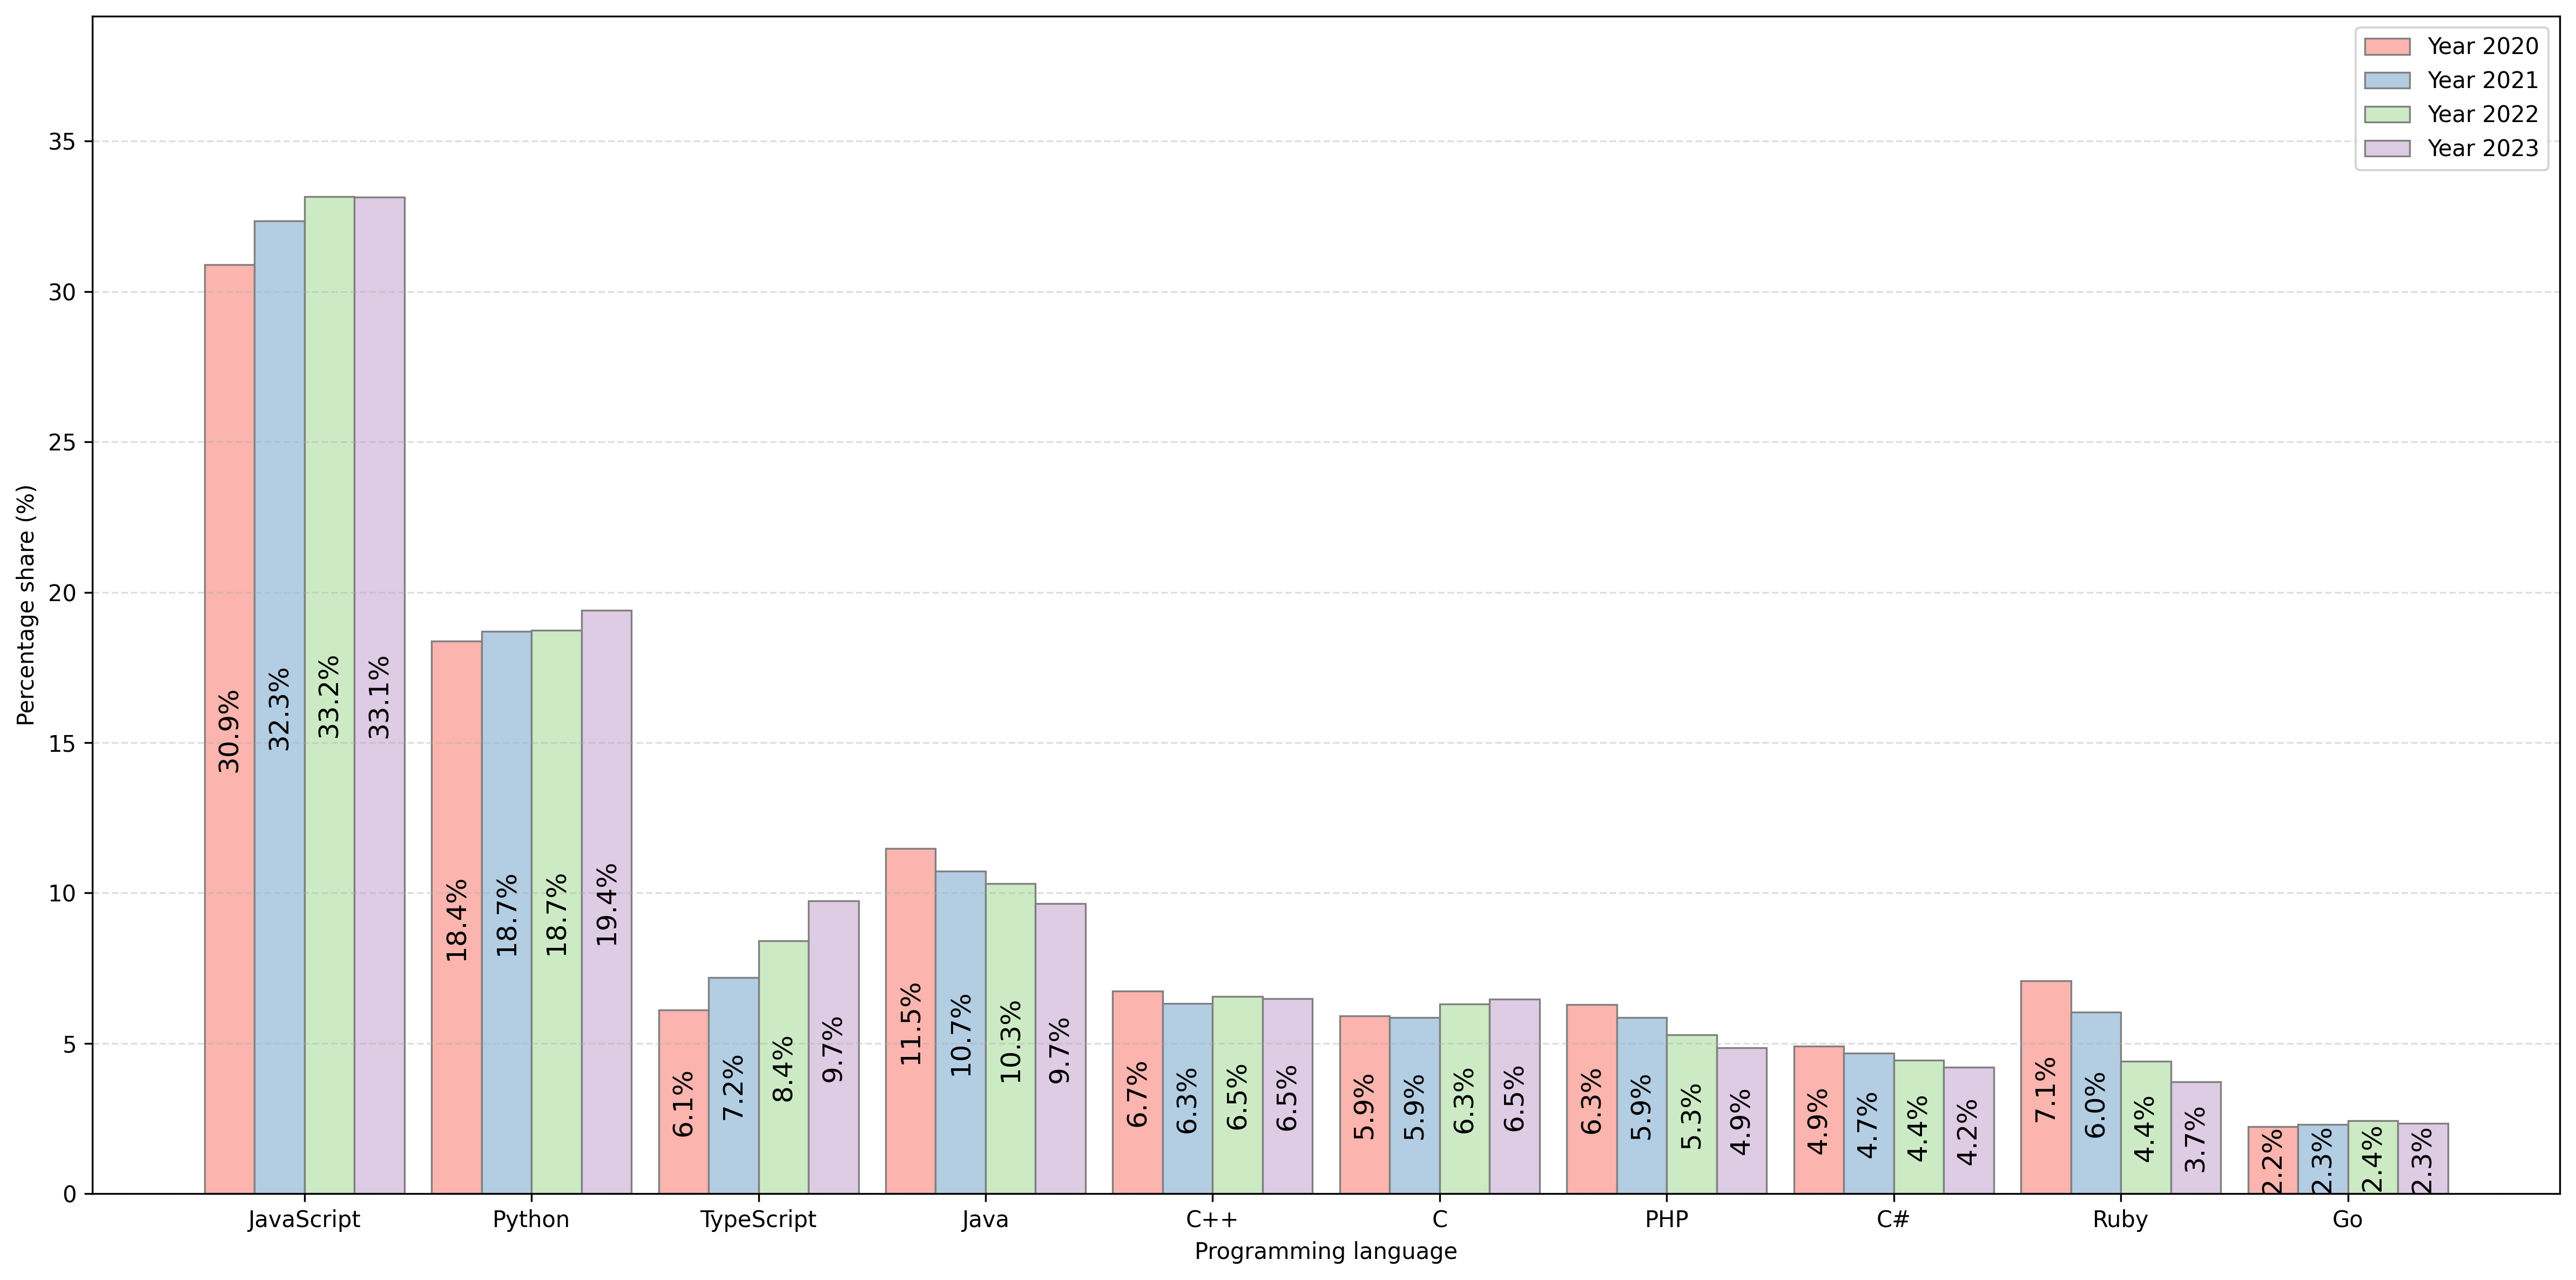
\includegraphics[width=0.85\textwidth]{language_distribution_gpt_available_2020_2023.png}
\caption*{\small Figura 1 de la tesis: países CON ChatGPT}
\end{figure}

\begin{lectura}{Qué muestran}
Estas figuras son \textbf{gráficos de barras agrupadas} donde:
\begin{itemize}[leftmargin=*]
  \item Cada lenguaje (eje horizontal) tiene 4 barras —una por año (2020, 2021, 2022, 2023).
  \item La altura de cada barra es el \textbf{porcentaje del total de \textit{unique pushers}} que ese lenguaje representa en ese año.
  \item Figura 1 = países con ChatGPT; Figura 2 = países sin ChatGPT.
\end{itemize}
\end{lectura}

\textbf{Cómo leerlos.} JavaScript ocupa la barra más alta porque es el lenguaje más usado. Si su barra de 2023 es más alta que la de 2020, significa que JavaScript ganó participación. Si bajó, perdió.

\textbf{Lo que se observa:} En los países CON ChatGPT (Figura 1), JavaScript crece de 30,9\,\% a 33,1\,\% y TypeScript crece de 6,1\,\% a 9,7\,\%. En los países SIN ChatGPT (Figura 2), JavaScript se mantiene estable (30,5\,\% $\rightarrow$ 30,0\,\%) y Java cae con más fuerza. Esta diferencia en la dinámica de \textit{composición} es una primera pista visual de que algo cambió.

% ════════════════════════════════════════════════════════════════════════════
\section{Las Figuras 3 y 4 (tendencias temporales)}

\begin{figure}[H]
\centering
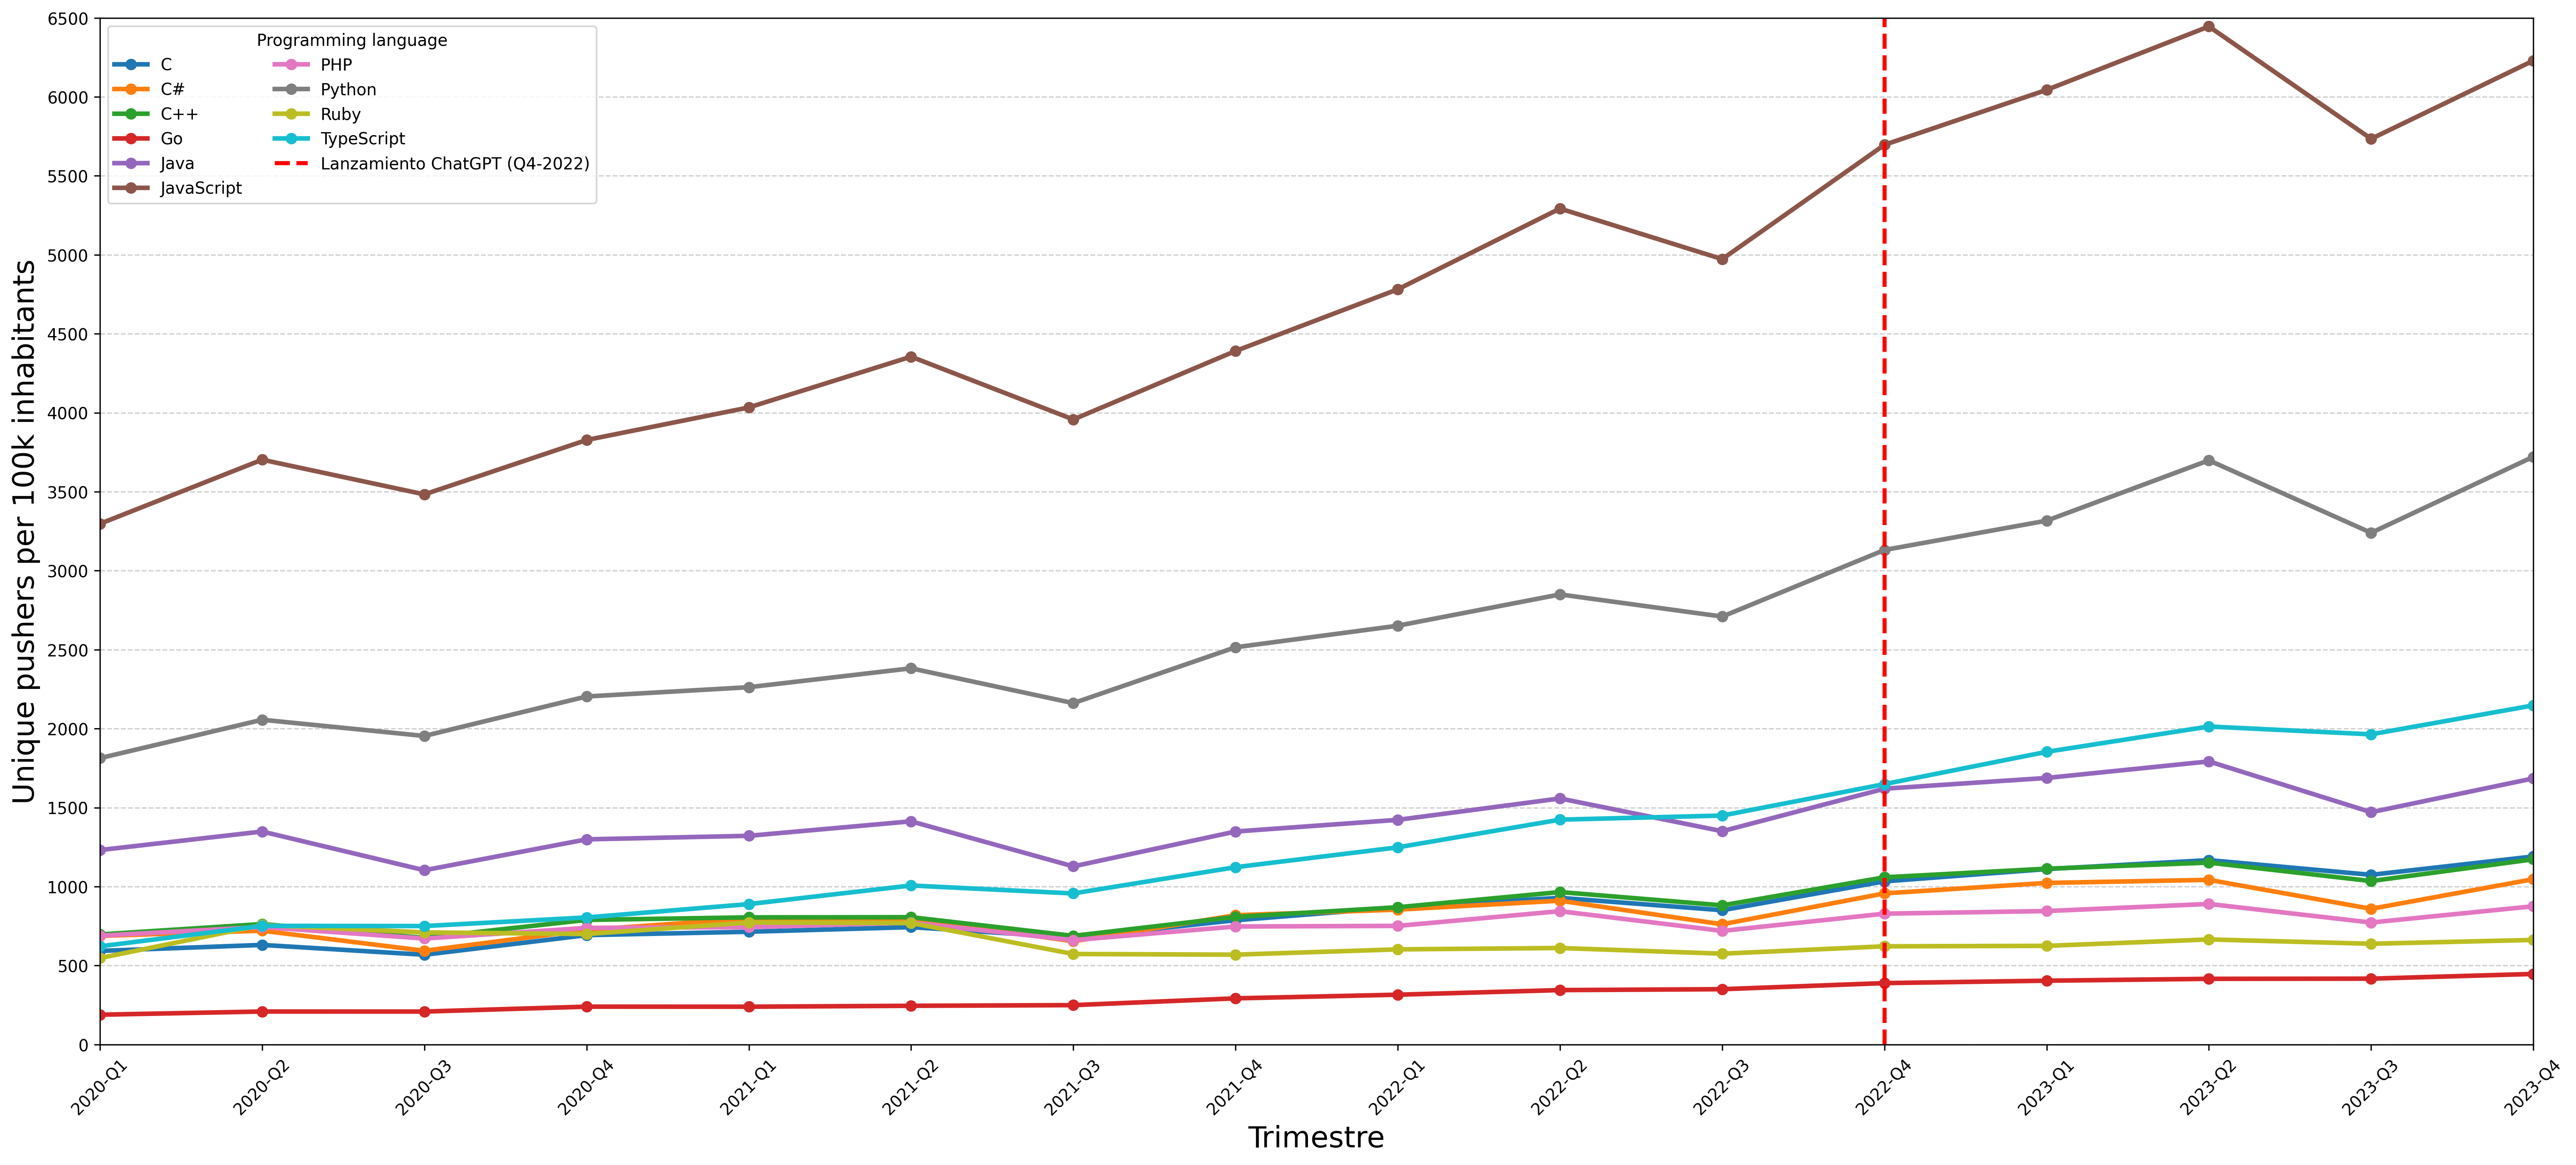
\includegraphics[width=0.95\textwidth]{language_trend_gpt_countries_2020_2023.png}
\caption*{\small Figura 3 de la tesis: tendencias en países CON ChatGPT}
\end{figure}

\begin{lectura}{Qué muestran}
Series de tiempo trimestrales del número de \textit{unique pushers} por cada 100k habitantes:
\begin{itemize}[leftmargin=*]
  \item Eje horizontal: 16 trimestres (Q1-2020 a Q4-2023).
  \item Eje vertical: \textit{unique pushers} por 100k.
  \item Una línea por lenguaje.
  \item \textbf{La línea vertical roja punteada} marca Q4-2022 (lanzamiento de ChatGPT).
\end{itemize}
\end{lectura}

\textbf{Cómo leerlas.} Observa cualquier lenguaje, por ejemplo Python (línea naranja). Si justo después de la línea roja vertical su trayectoria se vuelve más empinada (sube más rápido que antes), eso es consistente con un \textbf{efecto positivo del tratamiento}. Si la pendiente no cambia, no hay efecto visible. Si ya venía subiendo igual, podría tratarse de tendencia previa, no de efecto causal —pero eso lo decide la econometría, no el ojo.

Comparando Figuras 3 y 4: en los países CON ChatGPT (Fig.~3), las pendientes de JavaScript y Python se aceleran visiblemente después de Q4-2022. En los países SIN ChatGPT (Fig.~4), las pendientes son más planas. Esta divergencia visual sustenta el efecto que después cuantifican los métodos econométricos.

% ════════════════════════════════════════════════════════════════════════════
\section{Las Figuras 5--14 (tendencias y pesos por lenguaje)}

Estas son las figuras más densas de la tesis. Cada una tiene \textbf{seis paneles} (a, b, c, d, e, f) que muestran cómo cada método construyó su contrafactual para un lenguaje específico. Hay una figura por cada uno de los 10 lenguajes.

\begin{lectura}{La estructura de cada figura}
\begin{itemize}[leftmargin=*]
  \item \textbf{Panel (a) Tendencias DiD:} línea azul = grupo tratado promedio, línea roja = grupo de control promedio. Si las dos líneas no son paralelas en el pre-período, el supuesto DiD se viola.
  \item \textbf{Panel (b) Pesos DiD:} línea roja horizontal que indica peso uniforme $1/N_c$. Todos los controles pesan igual.
  \item \textbf{Panel (c) Tendencias CS:} línea azul = tratado real, línea roja = ``tratado sintético'' construido con pesos. Si las líneas se superponen bien en el pre-período, CS funciona.
  \item \textbf{Panel (d) Pesos CS:} cada punto representa un país de control. \textbf{Puntos azules} = pesos significativos (donantes importantes); \textbf{puntos rojos} = pesos negligibles (donantes que aportan poco al contrafactual, no necesariamente cero exacto). Tamaño del punto $\propto$ magnitud del peso.
  \item \textbf{Panel (e) Tendencias SDiD:} igual que (c) pero usando los pesos del método SDiD. \textbf{Área sombreada} muestra los pesos temporales: cuanto más cerca de Q4-2022, mayor peso.
  \item \textbf{Panel (f) Pesos SDiD:} igual lectura que (d).
\end{itemize}
\end{lectura}

\textbf{Ejemplo: Python (Figura 7 de la tesis, paneles e y f).} A continuación se muestran los dos paneles que produce el método SDiD para el lenguaje Python: a la izquierda el panel de \textit{tendencias} (panel e) y a la derecha el panel de \textit{pesos} (panel f). Ambos se leen en conjunto.

\begin{figure}[H]
\centering
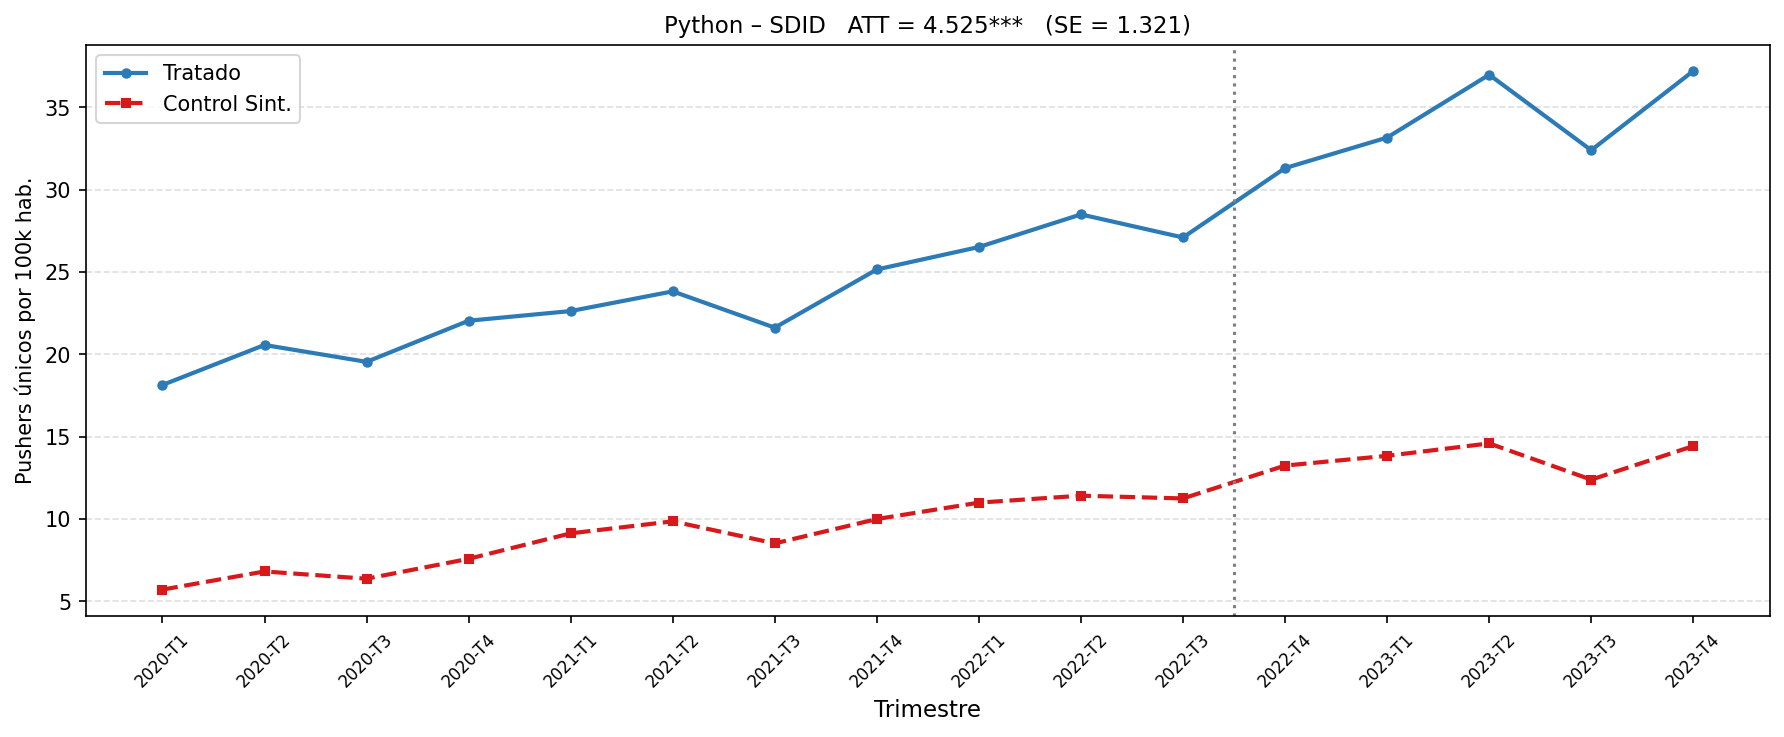
\includegraphics[width=0.95\textwidth]{Pythonsdidtrends12.png}
\caption*{\small \textbf{Panel (e) Tendencias estimadas SDiD --- Python.} Línea azul = grupo tratado (130 países promediados); línea roja = control sintético (28 países de control ponderados). Antes de Q4-2022 las dos líneas se superponen casi perfectamente, lo que valida el contrafactual. Después de Q4-2022 la línea azul se aleja por encima de la roja: ese gap es el efecto estimado (ATT = $4{,}525$).}
\end{figure}

\begin{figure}[H]
\centering
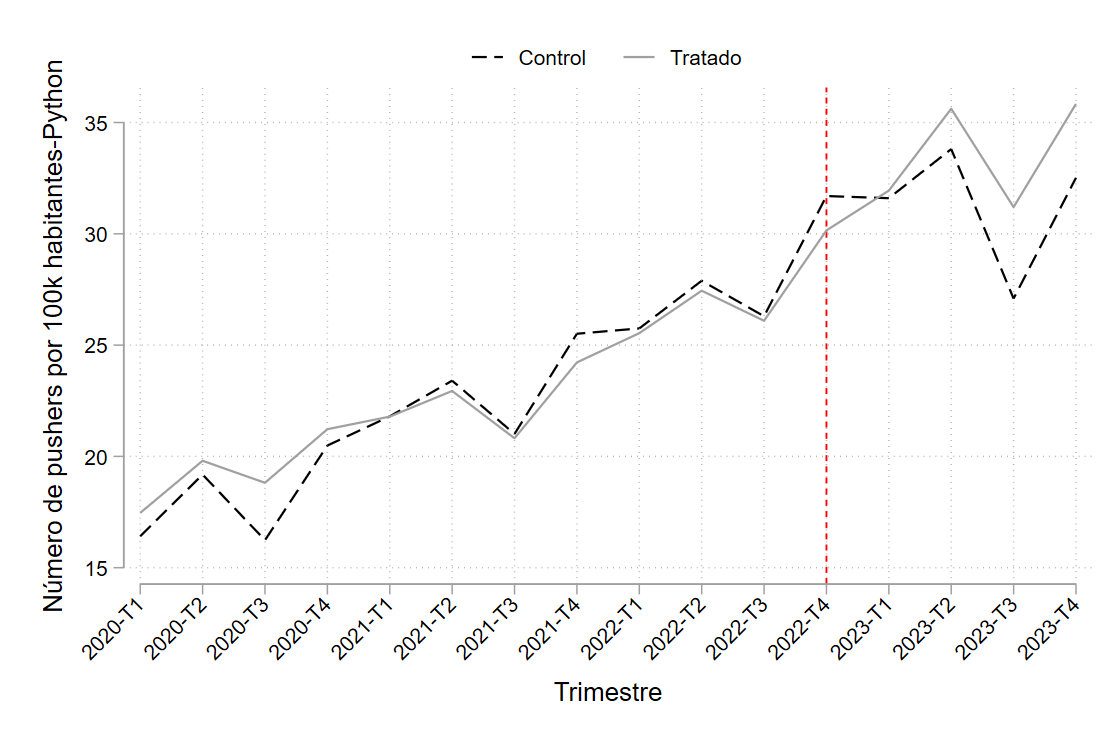
\includegraphics[width=0.95\textwidth]{Pythonsdidweights12.png}
\caption*{\small \textbf{Panel (f) Pesos SDiD --- Python.} Cada punto representa uno de los 29 países de control. Los azules grandes (CN, RU, IR) son los donantes con peso significativo. Los puntos rojos chicos son países cuyo peso es inferior al 30\,\% del peso uniforme $1/29 \approx 0{,}034$, es decir, donantes que aportan muy poco al contrafactual.}
\end{figure}

\textbf{Qué buscar al leer los dos paneles juntos.}

\begin{enumerate}[leftmargin=*]
  \item \textbf{En el panel de tendencias (a/c/e):} ¿Las dos líneas se superponen bien ANTES de Q4-2022? Si sí, el método construyó un buen contrafactual ---el control sintético reproduce al tratado en el pre-período. ¿Se separan DESPUÉS de Q4-2022? Si sí, hay un efecto visible cuya magnitud es la distancia vertical entre las líneas (eje $y$ en unique pushers por 100 mil habitantes).
  \item \textbf{En el panel de pesos (b/d/f):} ¿Cuántos puntos azules (significativos) hay? Pocos puntos azules significa que el contrafactual depende fuertemente de unos pocos donantes ---menos robusto, porque si alguno de ellos es atípico la estimación se contamina. Muchos puntos azules con tamaños parecidos significa contrafactual diversificado y estable.
  \item \textbf{La línea roja horizontal en los paneles de pesos} indica el peso promedio. Si los puntos azules quedan claramente por encima de ella, son donantes que contribuyen más que un país ``promedio'' del pool. La línea punteada morada marca el peso uniforme $1/N_c$ ($\approx 0{,}034$ para 29 países), que es el peso que cada control recibiría en un DiD clásico.
\end{enumerate}

\begin{warning}{Un punto rojo no significa peso cero}
Los puntos rojos en los paneles de pesos representan países con \textbf{peso negligible}, definido en el código como ``peso menor al 30\,\% del peso uniforme $1/N_c$''. Esto NO significa que el peso sea exactamente cero ---son valores cercanos a cero pero técnicamente positivos. La distinción visual entre azul y rojo es una convención que el código usa para resaltar qué donantes mandan en la construcción del contrafactual.
\end{warning}

% ════════════════════════════════════════════════════════════════════════════
\section{El Cuadro 3 (resultados principales)}

Este es el cuadro central de la tesis. Resume todos los resultados de los tres métodos para los 10 lenguajes.

\begin{lectura}{Estructura del Cuadro 3}
\begin{itemize}[leftmargin=*]
  \item \textbf{Filas:} los 10 lenguajes.
  \item \textbf{Columnas:} DID, SC (= CS), SDID, Observaciones, Baseline Mean.
  \item Cada celda tiene \textbf{dos números}: el coeficiente estimado y, debajo entre paréntesis, el error estándar.
  \item \textbf{Las estrellas} indican significancia estadística: $*$ p$<$0,10 \quad $**$ p$<$0,05 \quad $***$ p$<$0,01.
  \item Decimales con coma (convención española): ``$8{,}303$'' significa 8,303 unique pushers, no 8.303.
\end{itemize}
\end{lectura}

\textbf{Cómo interpretar una celda.} Considera la fila JavaScript, columna SDID: aparece $8{,}303^{***}$ con $(3{,}180)$ debajo. Esto significa:

\begin{itemize}[leftmargin=*]
  \item \textbf{Efecto estimado (ATT):} $+8{,}303$ \textit{unique pushers} adicionales por cada 100k habitantes, atribuibles a la disponibilidad de ChatGPT.
  \item \textbf{Error estándar:} $3{,}180$. Para construir un intervalo de confianza aproximado al 95\,\%, se calcula $8{,}303 \pm 2 \times 3{,}180$, es decir $[1{,}94;\ 14{,}66]$.
  \item \textbf{Tres estrellas ($***$):} el p-valor es menor que 0,01, lo que significa que es muy poco probable que un efecto de esta magnitud apareciera por azar si el efecto verdadero fuera cero.
\end{itemize}

\textbf{La columna Baseline Mean.} Indica el promedio pre-tratamiento del grupo de control para ese lenguaje. Sirve para dar contexto: un efecto de $+8{,}303$ sobre un baseline de $36{,}571$ es un aumento relativo de aproximadamente $23\,\%$.

\textbf{Por qué tres métodos.} Cada método tiene supuestos distintos. Si los tres coinciden en signo y significancia, la conclusión es más sólida. Si uno difiere, hay que entender por qué. Por ejemplo, en Python el CS aparece sin significancia ($1{,}604$, SE $3{,}552$), mientras DiD y SDiD sí ($+7{,}688$ y $+4{,}525$, ambos con $***$): esto refleja que el CS puro tiene mayor varianza cuando la unidad tratada es agregada y heterogénea.

% ════════════════════════════════════════════════════════════════════════════
\section{Los Cuadros 4 y 5 (controles y restricción del pool de donantes)}

\subsection{Cuadro 4: con variables de control}

Misma estructura que Cuadro 3, pero antes de estimar, se ``descuenta'' del \textit{outcome} el efecto de dos variables de control del Banco Mundial: porcentaje de uso de computadora y porcentaje de uso de internet. La idea es: ¿el efecto sobrevive cuando controlamos por infraestructura digital?

\textbf{Por qué no se reporta como principal:} 19 países no tienen datos completos de estas variables, así que se imputaron como cero. Eso introduce sesgo. Por eso el Cuadro 3 (sin controles) es la especificación principal y el Cuadro 4 es robustez.

\subsection{Cuadro 5: con grupo de control restringido}

¿Qué pasa si excluimos del grupo de control a los seis ``censores severos de internet'' (China, Cuba, Irán, Bielorrusia, Rusia, Siria), clasificados como ``No Libres'' por Freedom House?

\textbf{Lo que muestra:} dos columnas SDiD —``completo'' (29 controles, igual que Cuadro 3) y ``restringido'' (23 controles tras excluir censores severos). Si los efectos son similares en ambas, los resultados no dependen de incluir estos países atípicos.

% ════════════════════════════════════════════════════════════════════════════
\section{El Cuadro 6 (placebos y leave-one-out)}

Este cuadro es la novedad metodológica más fuerte que se agregó a la tesis. Es la respuesta directa al pedido del jurado de fortalecer las pruebas de robustez del SDiD.

\begin{lectura}{Qué muestra}
Dos pruebas de robustez complementarias, por lenguaje:
\begin{itemize}[leftmargin=*]
  \item \textbf{Placebos in-space:} para cada uno de los 29 países de control, lo reasigno como ``tratado'' y veo qué efecto da el SDiD. Como esos países nunca recibieron ChatGPT, cualquier efecto que aparezca debería ser ruido. La distribución de 29 placebos por lenguaje es mi ``hipótesis nula empírica''.
  \item \textbf{Donor pool LOO (leave-one-out):} elimino un país de control del pool de donantes a la vez y reestimo el SDiD. Si el resultado depende mucho de un solo donante (China, por ejemplo), el rango LOO será amplio.
\end{itemize}
\end{lectura}

\textbf{Cómo interpretar cada columna del Cuadro 6:}

\begin{itemize}[leftmargin=*]
  \item \textbf{ATT observado:} es el mismo del Cuadro 3 (especificación principal SDiD).
  \item \textbf{Media placebos:} promedio de los 29 ATT placebo. Si tu tratamiento no tiene efecto, debería estar cerca de cero. Y de hecho lo está (todos cerca de 0).
  \item \textbf{p-valor placebo:} fracción de placebos cuyo $|\text{ATT}|$ es mayor o igual al $|\text{ATT}|$ observado. Si es chico ($<0{,}05$), significa que tu efecto es \textbf{atípico} respecto a la nula —respaldando la interpretación causal.
  \item \textbf{LOO mín / mediana / máx:} el rango de ATT que se obtiene al sacar cada donante. Si ese rango está siempre del mismo lado de cero (todos positivos), el efecto es estable. Si cruza cero, depende fuertemente de algún donante.
\end{itemize}

\textbf{Lo que el cuadro revela: tres niveles de fortaleza de evidencia.}

\begin{itemize}[leftmargin=*]
  \item \textbf{Evidencia fuerte} (p $\leq 0{,}05$): Go ($p = 0{,}034$), Ruby ($p = 0{,}034$).
  \item \textbf{Evidencia moderada} (p $\leq 0{,}10$): JavaScript ($p = 0{,}069$), Python ($p = 0{,}069$), TypeScript ($p = 0{,}069$).
  \item \textbf{Evidencia débil} (p $> 0{,}10$): C ($0{,}103$), Java ($0{,}103$), C++ ($0{,}138$), PHP ($0{,}172$), C\# ($0{,}207$).
\end{itemize}

Esto matiza la lectura del Cuadro 3: aunque los SE bootstrap del Cuadro 3 declaran significancia al 1\,\% para C, C++ y Java, las pruebas placebo muestran que ese efecto podría no distinguirse del ruido inherente al grupo de control. Honestidad metodológica.

% ════════════════════════════════════════════════════════════════════════════
\section{La Figura 15 (forest plot de robustez)}

\begin{figure}[H]
\centering
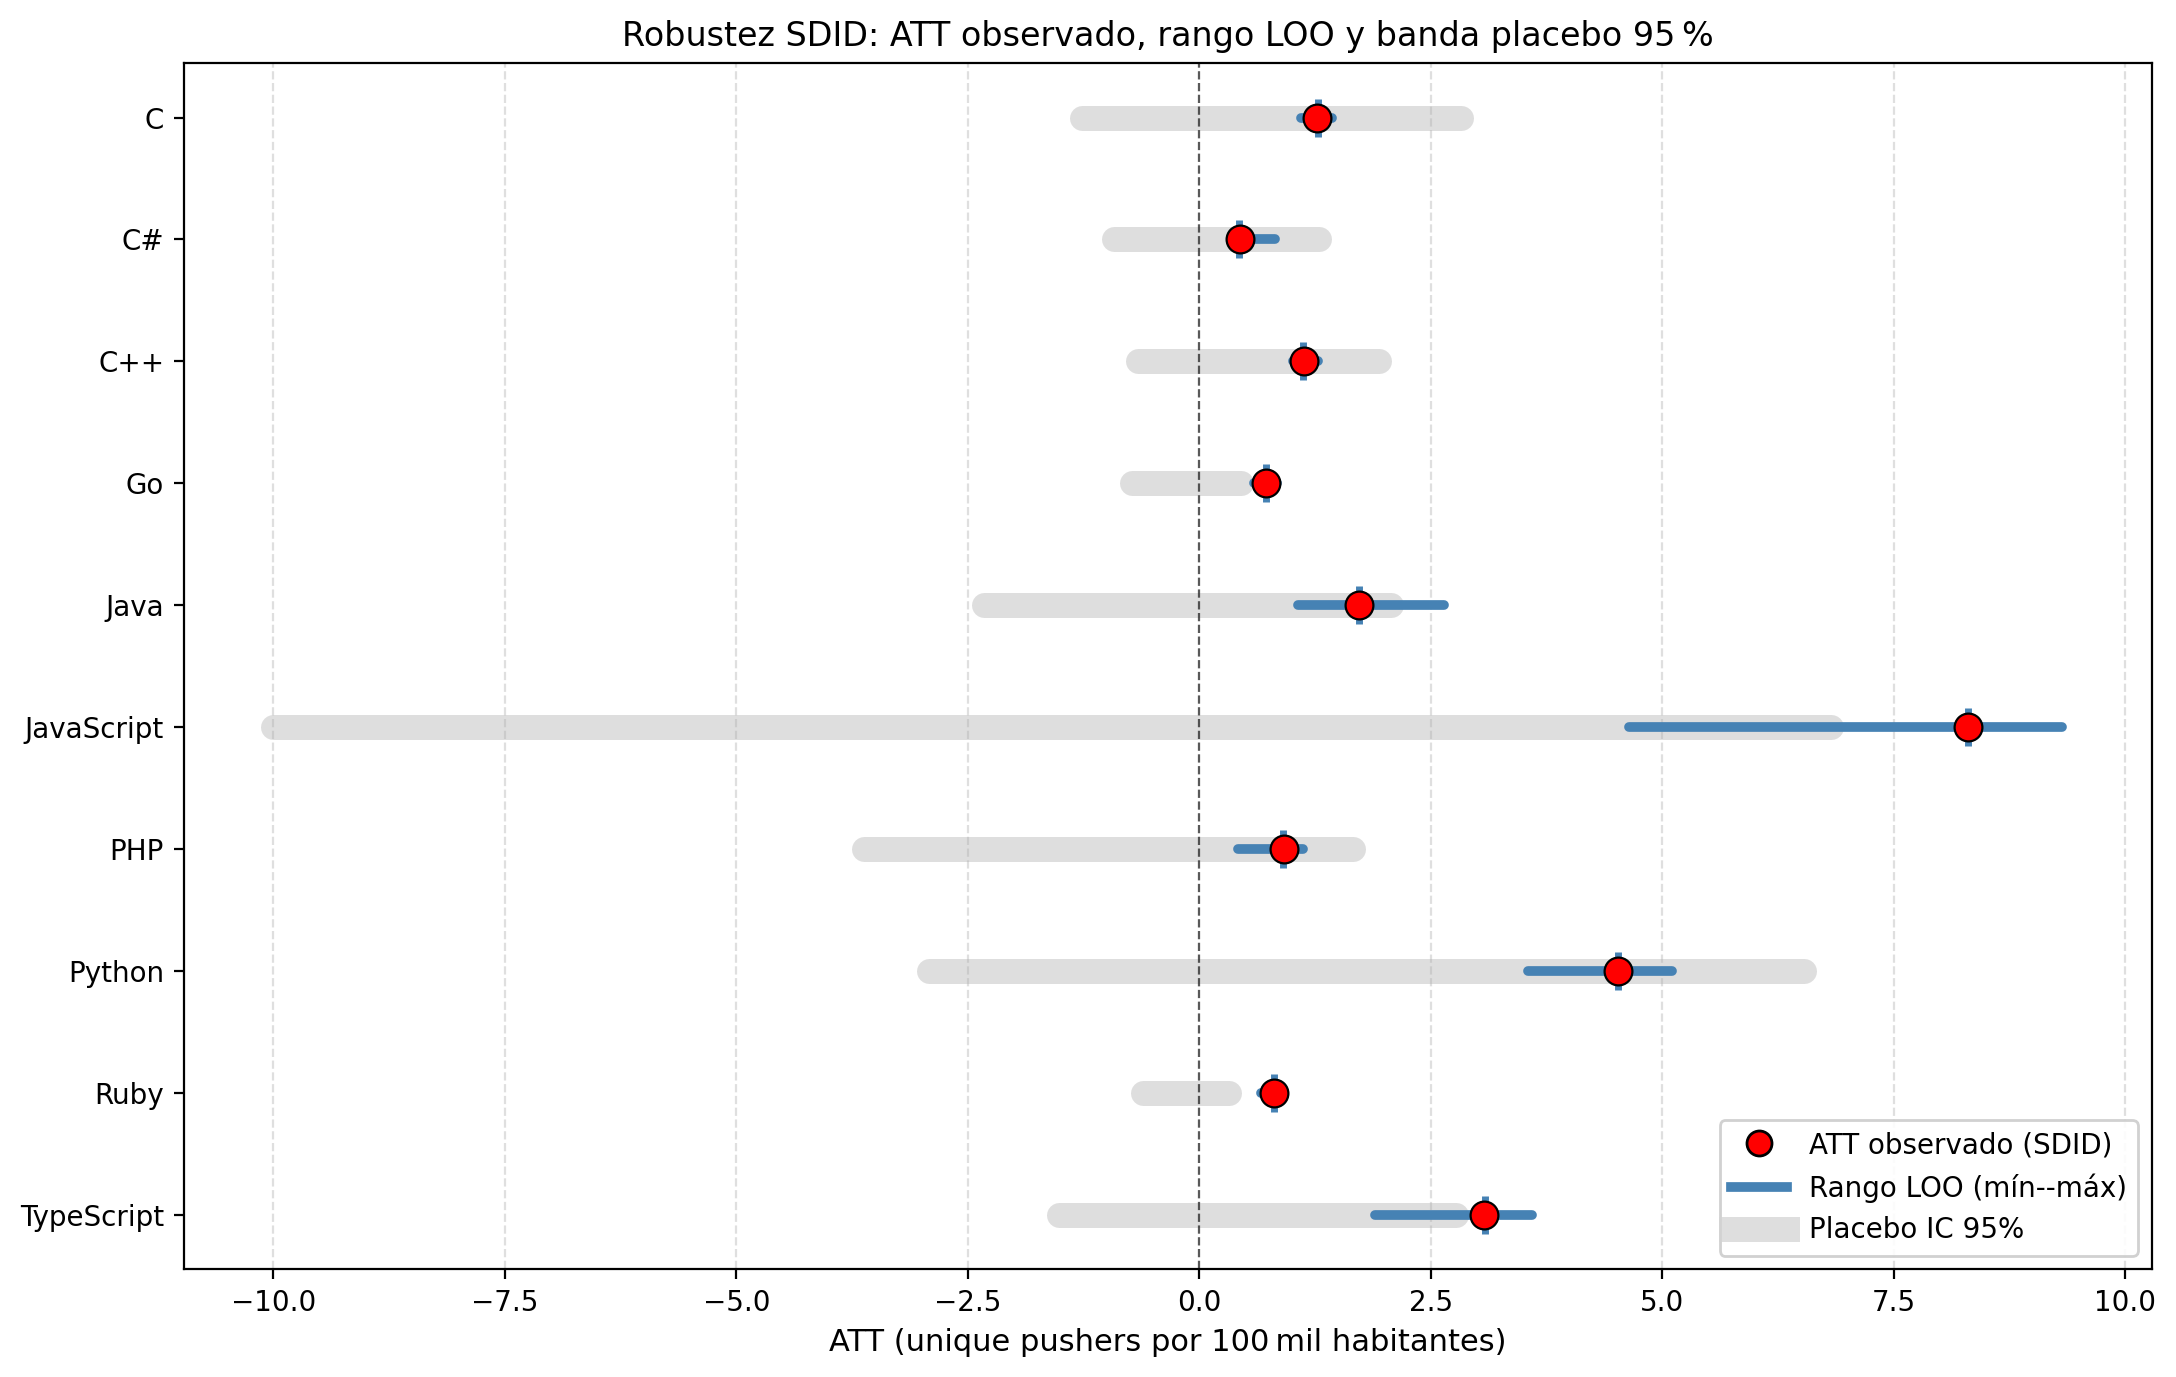
\includegraphics[width=\textwidth]{robustness_forest_plot.png}
\caption*{\small Figura 15 de la tesis: forest plot de robustez SDID}
\end{figure}

\begin{lectura}{Qué muestra}
Un resumen visual del Cuadro 6 para los 10 lenguajes a la vez:
\begin{itemize}[leftmargin=*]
  \item \textbf{Punto rojo:} el ATT observado (estimación principal del SDiD).
  \item \textbf{Barra azul:} el rango \textit{leave-one-out} (mín--máx al eliminar cada donante).
  \item \textbf{Banda gris:} intervalo de confianza al 95\,\% de los 29 ATT placebo.
  \item \textbf{Línea vertical negra punteada:} el cero.
\end{itemize}
\end{lectura}

\textbf{Cómo interpretarla.} Para cada lenguaje, revisa tres cosas:

\begin{enumerate}[leftmargin=*]
  \item ¿El punto rojo (ATT observado) está \textbf{fuera de la banda gris} (placebos)? Si sí, el efecto es atípico respecto a la nula $\rightarrow$ evidencia causal.
  \item ¿La barra azul (LOO) \textbf{no cruza el cero}? Si sí, ningún donante individual es capaz de invertir el signo del efecto $\rightarrow$ resultado robusto a la composición del pool.
  \item ¿El punto rojo está \textbf{cerca del centro} de la barra azul? Si sí, la estimación principal es representativa del rango LOO $\rightarrow$ no hay outliers conduciendo el resultado.
\end{enumerate}

\textbf{Lo que ves visualmente:} JavaScript, Python y TypeScript tienen puntos rojos fuera de la banda gris y barras LOO bien arriba de cero. C\#, PHP y otros tienen el punto rojo dentro o muy cerca de la banda gris —ahí está el origen de los p-valores placebo altos.

% ════════════════════════════════════════════════════════════════════════════
\section{La Figura 16 (distribución placebo por lenguaje)}

\begin{figure}[H]
\centering
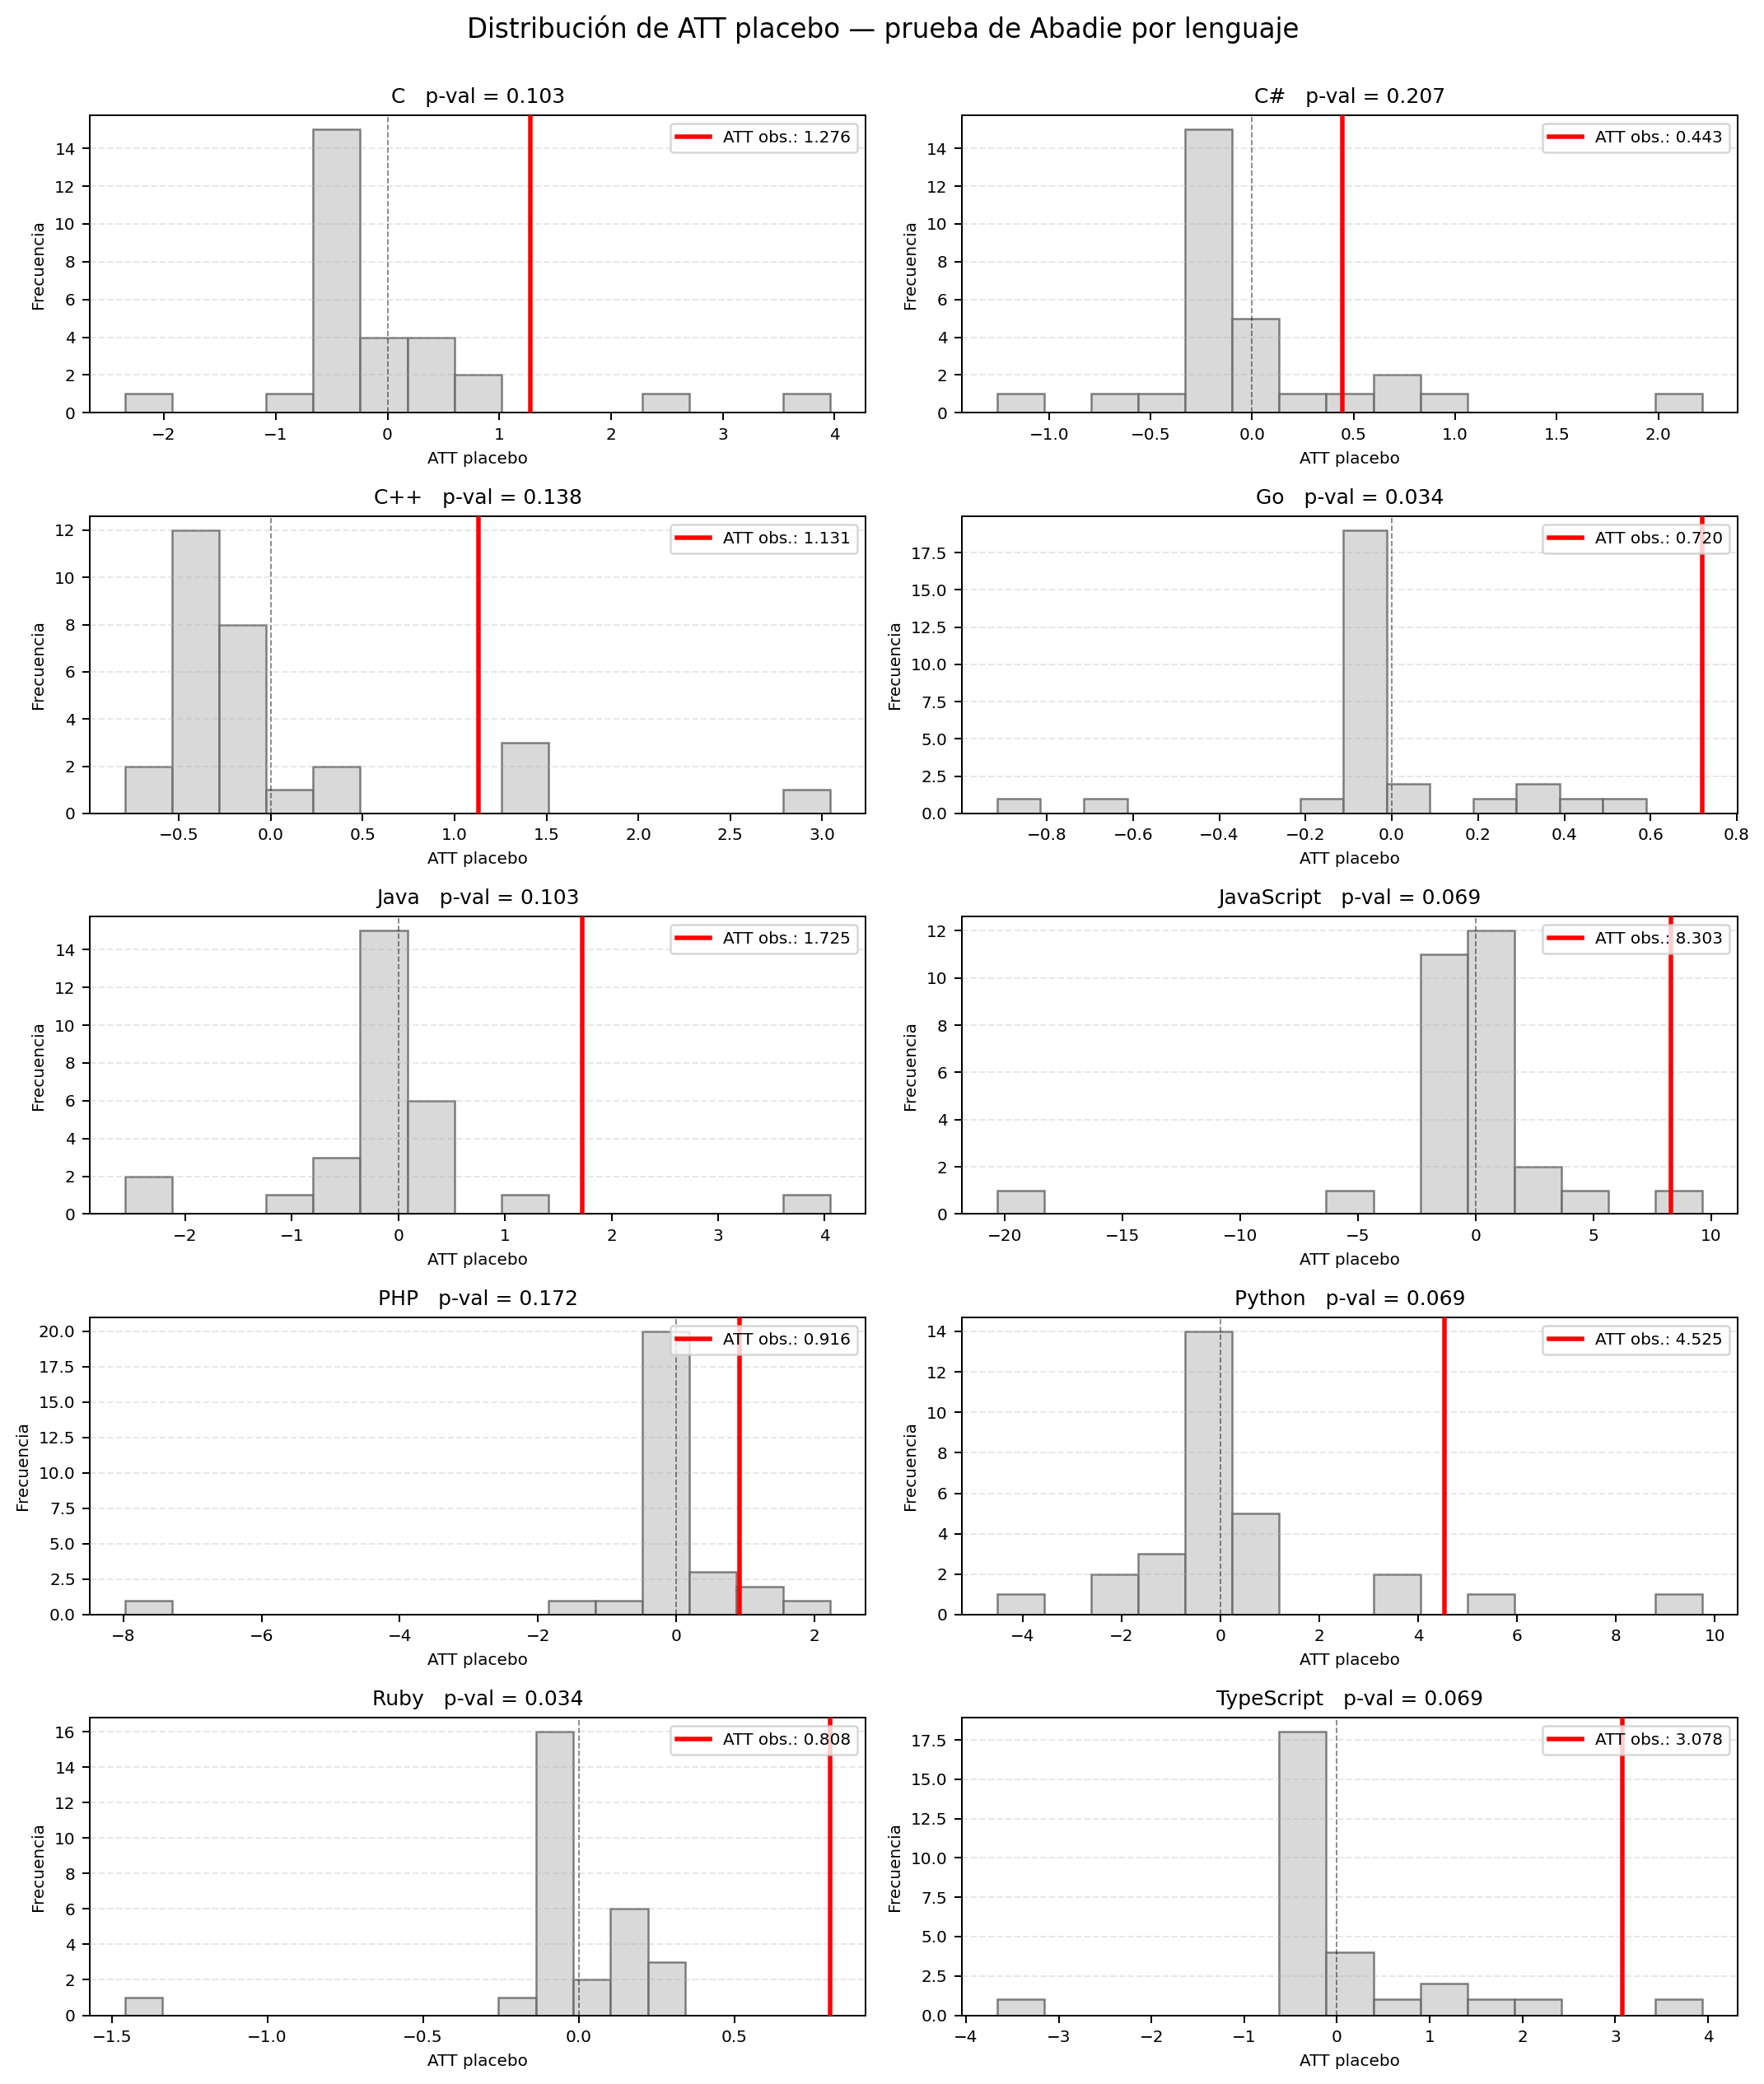
\includegraphics[width=0.95\textwidth]{placebo_distribution_panel.png}
\caption*{\small Figura 16 de la tesis: histogramas de ATT placebo por lenguaje}
\end{figure}

\begin{lectura}{Qué muestra}
10 histogramas (uno por lenguaje), cada uno con:
\begin{itemize}[leftmargin=*]
  \item \textbf{Barras grises:} la distribución de los 29 ATT placebo.
  \item \textbf{Línea roja vertical:} el ATT observado (estimación principal).
  \item \textbf{En el título:} el p-valor placebo.
\end{itemize}
\end{lectura}

\textbf{Cómo interpretarlo.} Para cada panel, la pregunta es: ``¿Qué tan lejos a la derecha (o izquierda) está la línea roja respecto a la mayoría de las barras grises?''

\begin{itemize}[leftmargin=*]
  \item Si la línea roja cae \textbf{en la cola} de la distribución gris $\rightarrow$ el efecto observado es raro bajo la nula $\rightarrow$ evidencia causal.
  \item Si la línea roja cae \textbf{en el centro} de las barras grises $\rightarrow$ el efecto observado es indistinguible del ruido placebo $\rightarrow$ evidencia débil.
\end{itemize}

Observa Go y Ruby (p = 0,034): la línea roja está claramente afuera del grueso de las placebos. Observa C\# (p = 0,207): la línea roja está \textbf{dentro} de la distribución placebo —el efecto observado podría ser ruido.

% ════════════════════════════════════════════════════════════════════════════
\section{La Figura 17 (línea de tiempo)}

\begin{figure}[H]
\centering
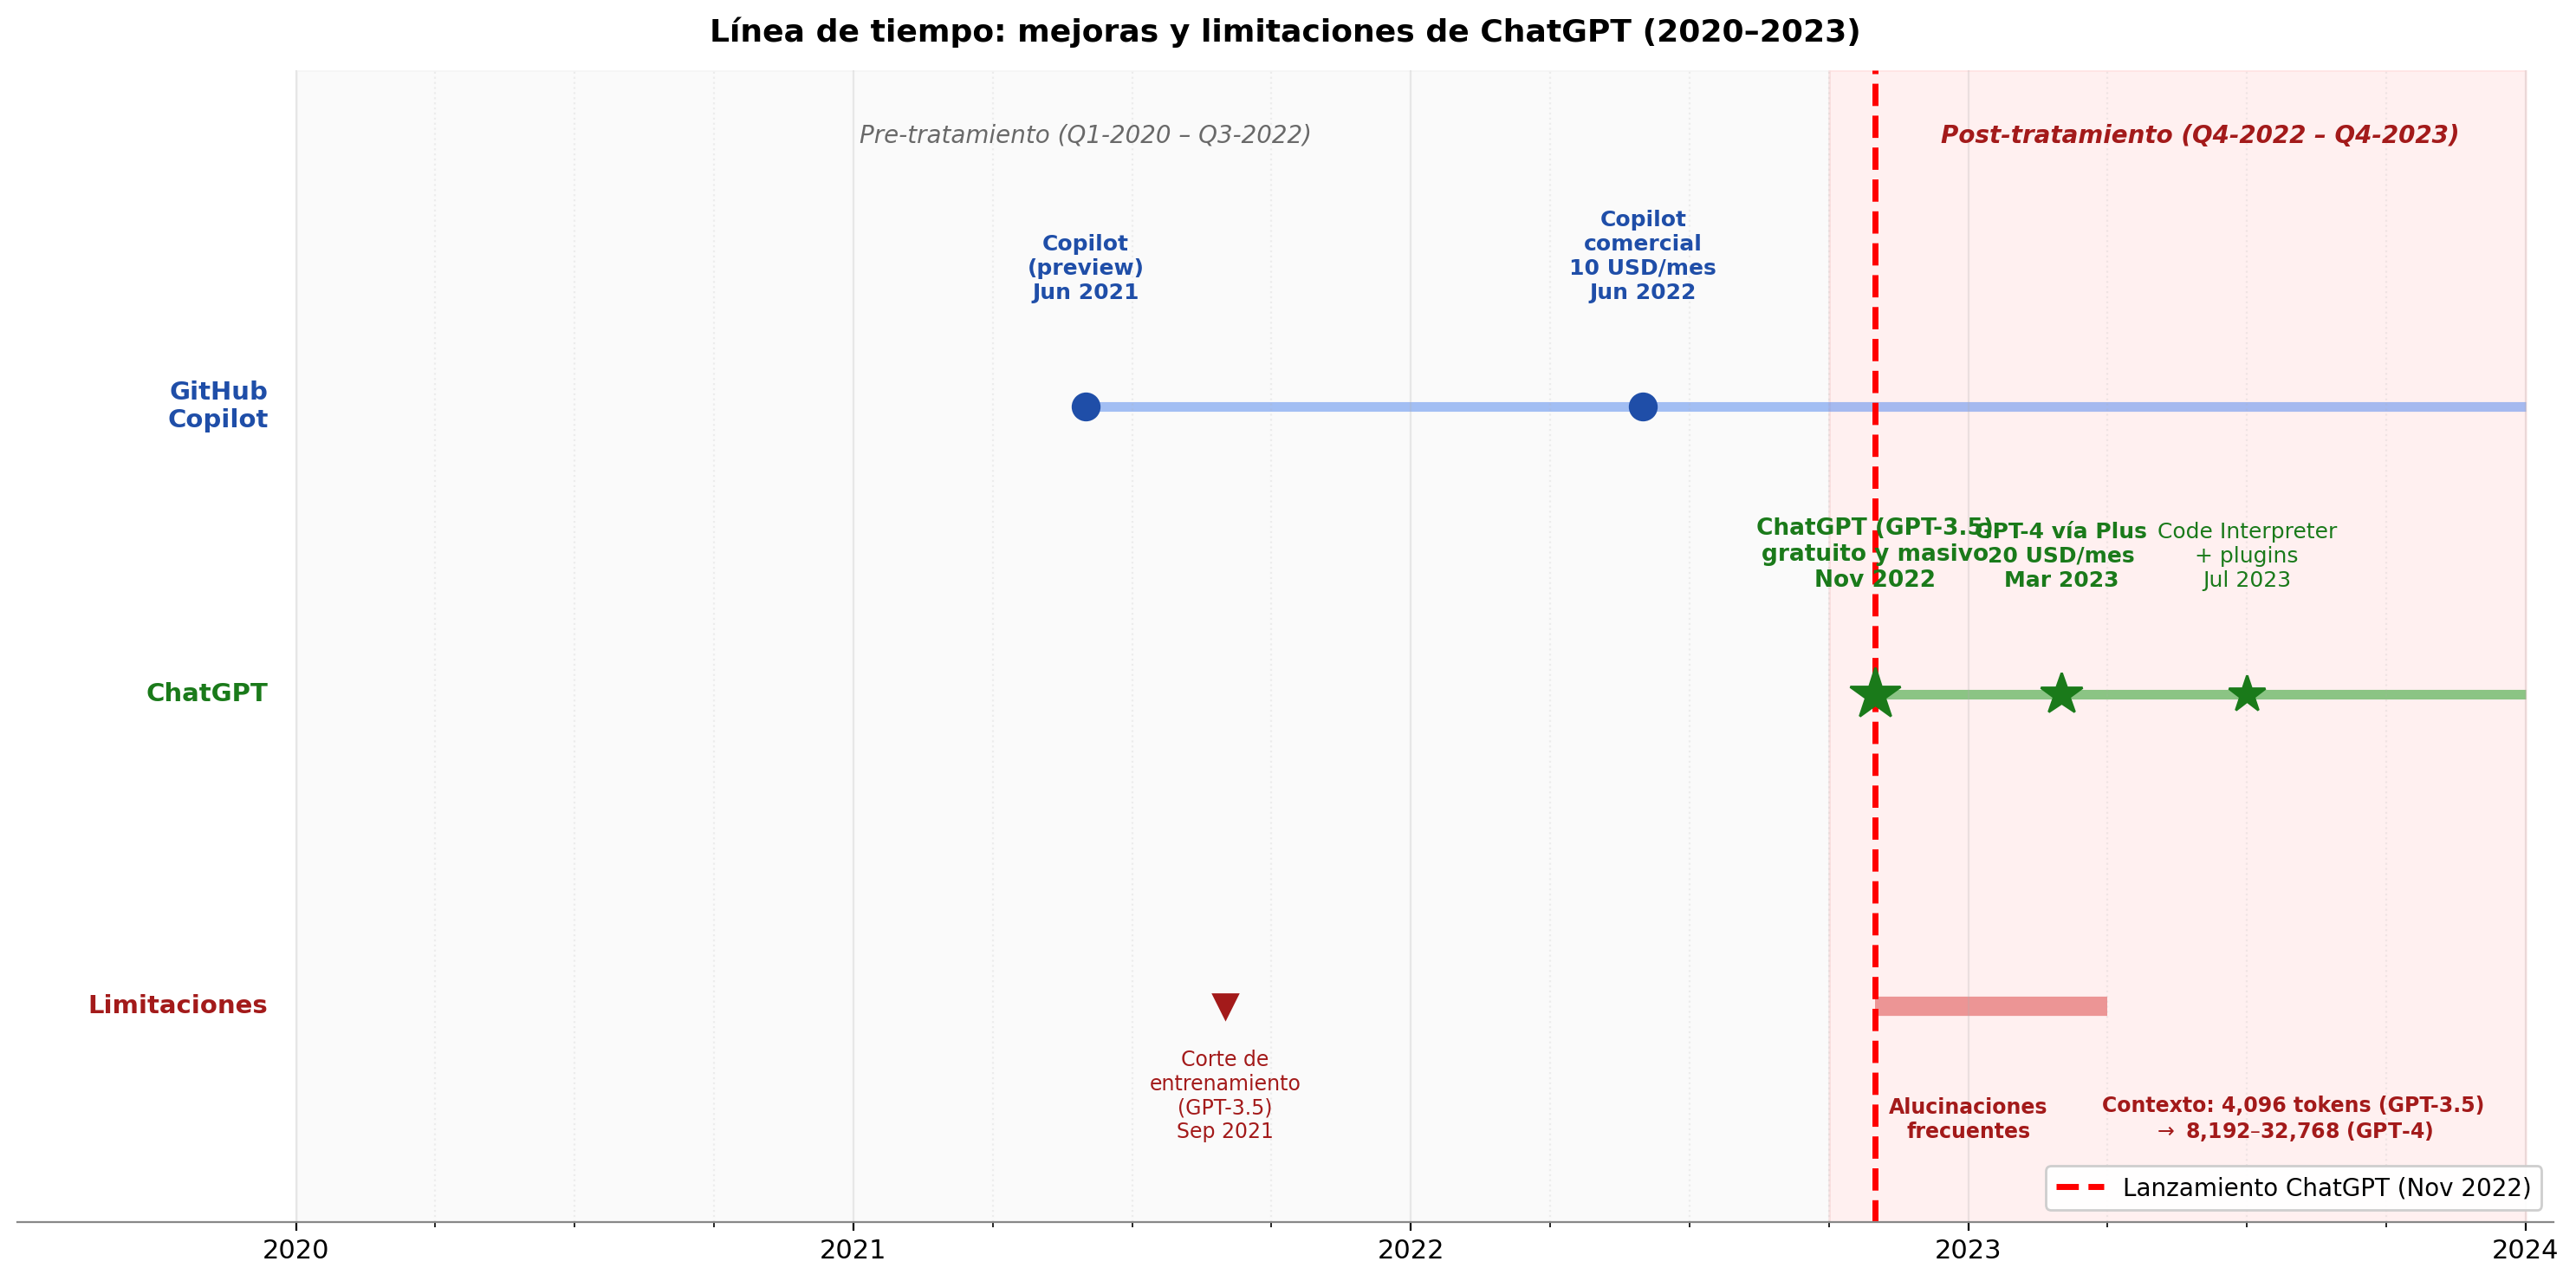
\includegraphics[width=\textwidth]{chatgpt_timeline.png}
\caption*{\small Figura 17 de la tesis: línea de tiempo ChatGPT (2020--2023)}
\end{figure}

\begin{lectura}{Qué muestra}
Tres carriles (\textit{swim lanes}) horizontales:
\begin{itemize}[leftmargin=*]
  \item \textbf{Azul (GitHub Copilot):} preview Jun 2021, comercial Jun 2022.
  \item \textbf{Verde (ChatGPT):} GPT-3.5 Nov 2022 (gratuito, masivo) $\rightarrow$ GPT-4 Mar 2023 (premium 20 USD/mes) $\rightarrow$ Code Interpreter Jul 2023.
  \item \textbf{Rojo (Limitaciones):} barras que muestran la \textbf{duración} de cada limitación —corte de entrenamiento (Sep 2021), alucinaciones frecuentes (Nov 2022--Abr 2023), ventana de contexto restringida.
\end{itemize}
La \textbf{línea vertical roja} en Nov 2022 marca el inicio del tratamiento.
\end{lectura}

\textbf{Para qué sirve.} Muestra que la ventana postratamiento del estudio (Q4-2022 a Q4-2023) no fue homogénea: la primera mitad estuvo dominada por GPT-3.5 con sus limitaciones, mientras que en la segunda mitad GPT-4 estuvo disponible para usuarios premium. Esto justifica la advertencia, en la sección de implicaciones, de que el efecto estimado podría haber sido \textbf{no monotónico en el corto plazo}.

% ════════════════════════════════════════════════════════════════════════════
\section{Las Figuras 18--27 (análisis de evento)}

\begin{lectura}{Qué muestran}
Una figura por lenguaje (10 en total), todas en el Anexo C. Cada figura es un \textbf{event study} del SDiD:
\begin{itemize}[leftmargin=*]
  \item \textbf{Eje horizontal:} trimestres relativos al tratamiento (0 = Q4-2022). Valores negativos = pre-tratamiento, valores positivos = postratamiento.
  \item \textbf{Eje vertical:} \textit{gap} entre el grupo tratado y el control sintético, en cada trimestre.
  \item \textbf{Línea azul:} el gap estimado en cada trimestre.
  \item \textbf{Banda celeste:} intervalo de confianza al 95\,\% (bootstrap de 200 replicaciones).
  \item \textbf{Línea roja punteada vertical:} el inicio del tratamiento.
\end{itemize}
\end{lectura}

\textbf{Cómo interpretarlas.} Para que el SDiD sea creíble, la línea azul \textbf{antes} de la línea roja debe estar cerca de cero (pre-tendencias paralelas entre tratados y control sintético). \textbf{Después} de la línea roja, si la línea azul se aleja sistemáticamente de cero, hay efecto.

\textbf{Ejemplo crítico.} En JavaScript, la línea azul ya empieza a subir levemente \textbf{antes} de Q4-2022 —pre-tendencia creciente. Esto es la razón por la que en la tesis se advierte que el efecto causal para JavaScript debe interpretarse con cautela, a pesar de su alta significancia estadística.

% ════════════════════════════════════════════════════════════════════════════
\section{Resumen ejecutivo de los hallazgos}

\textbf{El estudio en 5 puntos:}

\begin{enumerate}[leftmargin=*]
  \item \textbf{La pregunta:} ¿Aumentó la actividad de desarrollo en GitHub en los países donde ChatGPT estuvo disponible?
  \item \textbf{El diseño:} Cuasi-experimento con 130 países tratados y 29 controles, ventana Q1-2020 a Q4-2023, 10 lenguajes.
  \item \textbf{Los métodos:} DiD (referencia), CS (contrafactual ponderado) y SDiD (combinación robusta, método principal).
  \item \textbf{Los resultados:} efectos positivos y significativos en JavaScript (+8,3), Python (+4,5), TypeScript (+3,1), Java (+1,7), C (+1,3), C++ (+1,1), PHP (+0,9), Ruby (+0,8) y Go (+0,7) \textit{unique pushers} por 100k habitantes. C\# no muestra efecto significativo.
  \item \textbf{La robustez:} placebos in-space y LOO estratifican la evidencia en tres niveles. Los lenguajes para los cuales la evidencia es \textbf{fuerte simultáneamente en las tres pruebas} (bootstrap + LOO + placebo) son los que la hipótesis priorizaba ex ante: Python, JavaScript y TypeScript, además de Go y Ruby. Esto refuerza la interpretación causal en estos casos y matiza los resultados para lenguajes con evidencia más débil.
\end{enumerate}

\textbf{Implicaciones prácticas:}

\begin{itemize}[leftmargin=*]
  \item ChatGPT no solo es popular —\textbf{cambia objetivamente la dinámica del ecosistema de desarrollo} en los países donde está disponible.
  \item El efecto es \textbf{heterogéneo por lenguaje}: más fuerte en lenguajes con vasta documentación técnica y representación en datos de entrenamiento (Python, JavaScript).
  \item \textbf{La política recomendada} (acceso gratuito a versiones avanzadas para desarrolladores junior + bonos por uso productivo de IA) se sustenta en este subconjunto robusto.
\end{itemize}

\textbf{Las limitaciones que reconoce la tesis:}

\begin{itemize}[leftmargin=*]
  \item La asignación al grupo de control no fue aleatoria (países con restricciones de internet tienen estructura tecnológica distinta).
  \item El uso de VPN puede haber contaminado el grupo de control.
  \item La ventana postratamiento es corta (solo 4 trimestres).
  \item La variable \textit{unique pushers} mide cantidad de desarrolladores, no calidad ni intensidad del código generado.
\end{itemize}

\vspace{2\baselineskip}

\begin{ideabox}{Para acordarte de una sola cosa}
La tesis no afirma que ChatGPT haya impactado a TODOS los lenguajes por igual. Afirma, con tres niveles de evidencia (bootstrap, LOO, placebos in-space), que el impacto es \textbf{robusto y positivo} en el subconjunto de lenguajes con mayor representación en los datos de entrenamiento del modelo —Python, JavaScript, TypeScript, Go y Ruby—, consistente con la hipótesis teórica anclada en Acemoglu \& Restrepo (2018) y Stigler (1961).
\end{ideabox}

\end{document}
